% GNUPLOT: LaTeX picture with Postscript
\begingroup
  \makeatletter
  \providecommand\color[2][]{%
    \GenericError{(gnuplot) \space\space\space\@spaces}{%
      Package color not loaded in conjunction with
      terminal option `colourtext'%
    }{See the gnuplot documentation for explanation.%
    }{Either use 'blacktext' in gnuplot or load the package
      color.sty in LaTeX.}%
    \renewcommand\color[2][]{}%
  }%
  \providecommand\includegraphics[2][]{%
    \GenericError{(gnuplot) \space\space\space\@spaces}{%
      Package graphicx or graphics not loaded%
    }{See the gnuplot documentation for explanation.%
    }{The gnuplot epslatex terminal needs graphicx.sty or graphics.sty.}%
    \renewcommand\includegraphics[2][]{}%
  }%
  \providecommand\rotatebox[2]{#2}%
  \@ifundefined{ifGPcolor}{%
    \newif\ifGPcolor
    \GPcolortrue
  }{}%
  \@ifundefined{ifGPblacktext}{%
    \newif\ifGPblacktext
    \GPblacktextfalse
  }{}%
  % define a \g@addto@macro without @ in the name:
  \let\gplgaddtomacro\g@addto@macro
  % define empty templates for all commands taking text:
  \gdef\gplbacktext{}%
  \gdef\gplfronttext{}%
  \makeatother
  \ifGPblacktext
    % no textcolor at all
    \def\colorrgb#1{}%
    \def\colorgray#1{}%
  \else
    % gray or color?
    \ifGPcolor
      \def\colorrgb#1{\color[rgb]{#1}}%
      \def\colorgray#1{\color[gray]{#1}}%
      \expandafter\def\csname LTw\endcsname{\color{white}}%
      \expandafter\def\csname LTb\endcsname{\color{black}}%
      \expandafter\def\csname LTa\endcsname{\color{black}}%
      \expandafter\def\csname LT0\endcsname{\color[rgb]{1,0,0}}%
      \expandafter\def\csname LT1\endcsname{\color[rgb]{0,1,0}}%
      \expandafter\def\csname LT2\endcsname{\color[rgb]{0,0,1}}%
      \expandafter\def\csname LT3\endcsname{\color[rgb]{1,0,1}}%
      \expandafter\def\csname LT4\endcsname{\color[rgb]{0,1,1}}%
      \expandafter\def\csname LT5\endcsname{\color[rgb]{1,1,0}}%
      \expandafter\def\csname LT6\endcsname{\color[rgb]{0,0,0}}%
      \expandafter\def\csname LT7\endcsname{\color[rgb]{1,0.3,0}}%
      \expandafter\def\csname LT8\endcsname{\color[rgb]{0.5,0.5,0.5}}%
    \else
      % gray
      \def\colorrgb#1{\color{black}}%
      \def\colorgray#1{\color[gray]{#1}}%
      \expandafter\def\csname LTw\endcsname{\color{white}}%
      \expandafter\def\csname LTb\endcsname{\color{black}}%
      \expandafter\def\csname LTa\endcsname{\color{black}}%
      \expandafter\def\csname LT0\endcsname{\color{black}}%
      \expandafter\def\csname LT1\endcsname{\color{black}}%
      \expandafter\def\csname LT2\endcsname{\color{black}}%
      \expandafter\def\csname LT3\endcsname{\color{black}}%
      \expandafter\def\csname LT4\endcsname{\color{black}}%
      \expandafter\def\csname LT5\endcsname{\color{black}}%
      \expandafter\def\csname LT6\endcsname{\color{black}}%
      \expandafter\def\csname LT7\endcsname{\color{black}}%
      \expandafter\def\csname LT8\endcsname{\color{black}}%
    \fi
  \fi
    \setlength{\unitlength}{0.0500bp}%
    \ifx\gptboxheight\undefined%
      \newlength{\gptboxheight}%
      \newlength{\gptboxwidth}%
      \newsavebox{\gptboxtext}%
    \fi%
    \setlength{\fboxrule}{0.5pt}%
    \setlength{\fboxsep}{1pt}%
\begin{picture}(5760.00,4320.00)%
    \gplgaddtomacro\gplbacktext{%
      \csname LTb\endcsname%%
      \put(682,704){\makebox(0,0)[r]{\strut{}$-2$}}%
      \put(682,1197){\makebox(0,0)[r]{\strut{}$0$}}%
      \put(682,1689){\makebox(0,0)[r]{\strut{}$2$}}%
      \put(682,2182){\makebox(0,0)[r]{\strut{}$4$}}%
      \put(682,2674){\makebox(0,0)[r]{\strut{}$6$}}%
      \put(682,3167){\makebox(0,0)[r]{\strut{}$8$}}%
      \put(682,3659){\makebox(0,0)[r]{\strut{}$10$}}%
      \put(3457,484){\makebox(0,0){\strut{}$\phi$}}%
      \put(3707,484){\makebox(0,0){\strut{}$e$}}%
      \put(3803,484){\makebox(0,0){\strut{}$\pi$}}%
      \put(814,484){\makebox(0,0){\strut{}$-10$}}%
      \put(1951,484){\makebox(0,0){\strut{}$-5$}}%
      \put(3089,484){\makebox(0,0){\strut{}$0$}}%
      \put(4226,484){\makebox(0,0){\strut{}$5$}}%
      \put(5363,484){\makebox(0,0){\strut{}$10$}}%
    }%
    \gplgaddtomacro\gplfronttext{%
      \csname LTb\endcsname%%
      \put(198,2181){\rotatebox{-270}{\makebox(0,0){\strut{}$Y$ axis}}}%
      \put(3088,154){\makebox(0,0){\strut{}$X$ axis}}%
      \put(3088,3989){\makebox(0,0){\strut{}Example}}%
      \csname LTb\endcsname%%
      \put(4376,3486){\makebox(0,0)[r]{\strut{}x with Lines}}%
      \csname LTb\endcsname%%
      \put(4376,3266){\makebox(0,0)[r]{\strut{}x*x with Points}}%
      \csname LTb\endcsname%%
      \put(4376,3046){\makebox(0,0)[r]{\strut{}sqrt(x) with Linespoints}}%
      \csname LTb\endcsname%%
      \put(4376,2826){\makebox(0,0)[r]{\strut{}sin(x) with Impulse}}%
    }%
    \gplbacktext
    \put(0,0){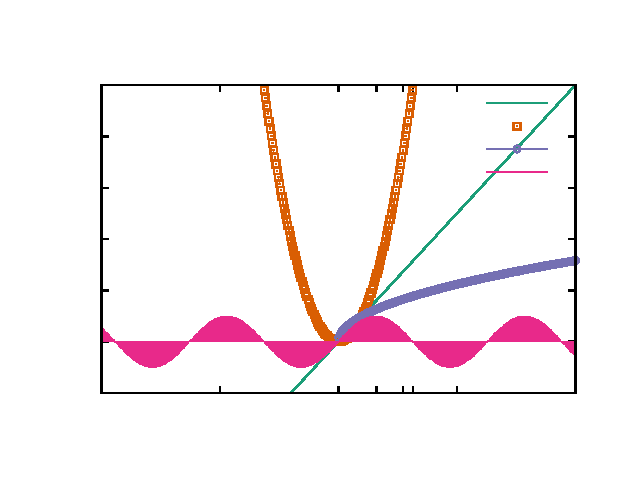
\includegraphics{figures/baseline2/plot}}%
    \gplfronttext
  \end{picture}%
\endgroup
